\chapter{轮子}
\begin{figure}[htbp]
\centering
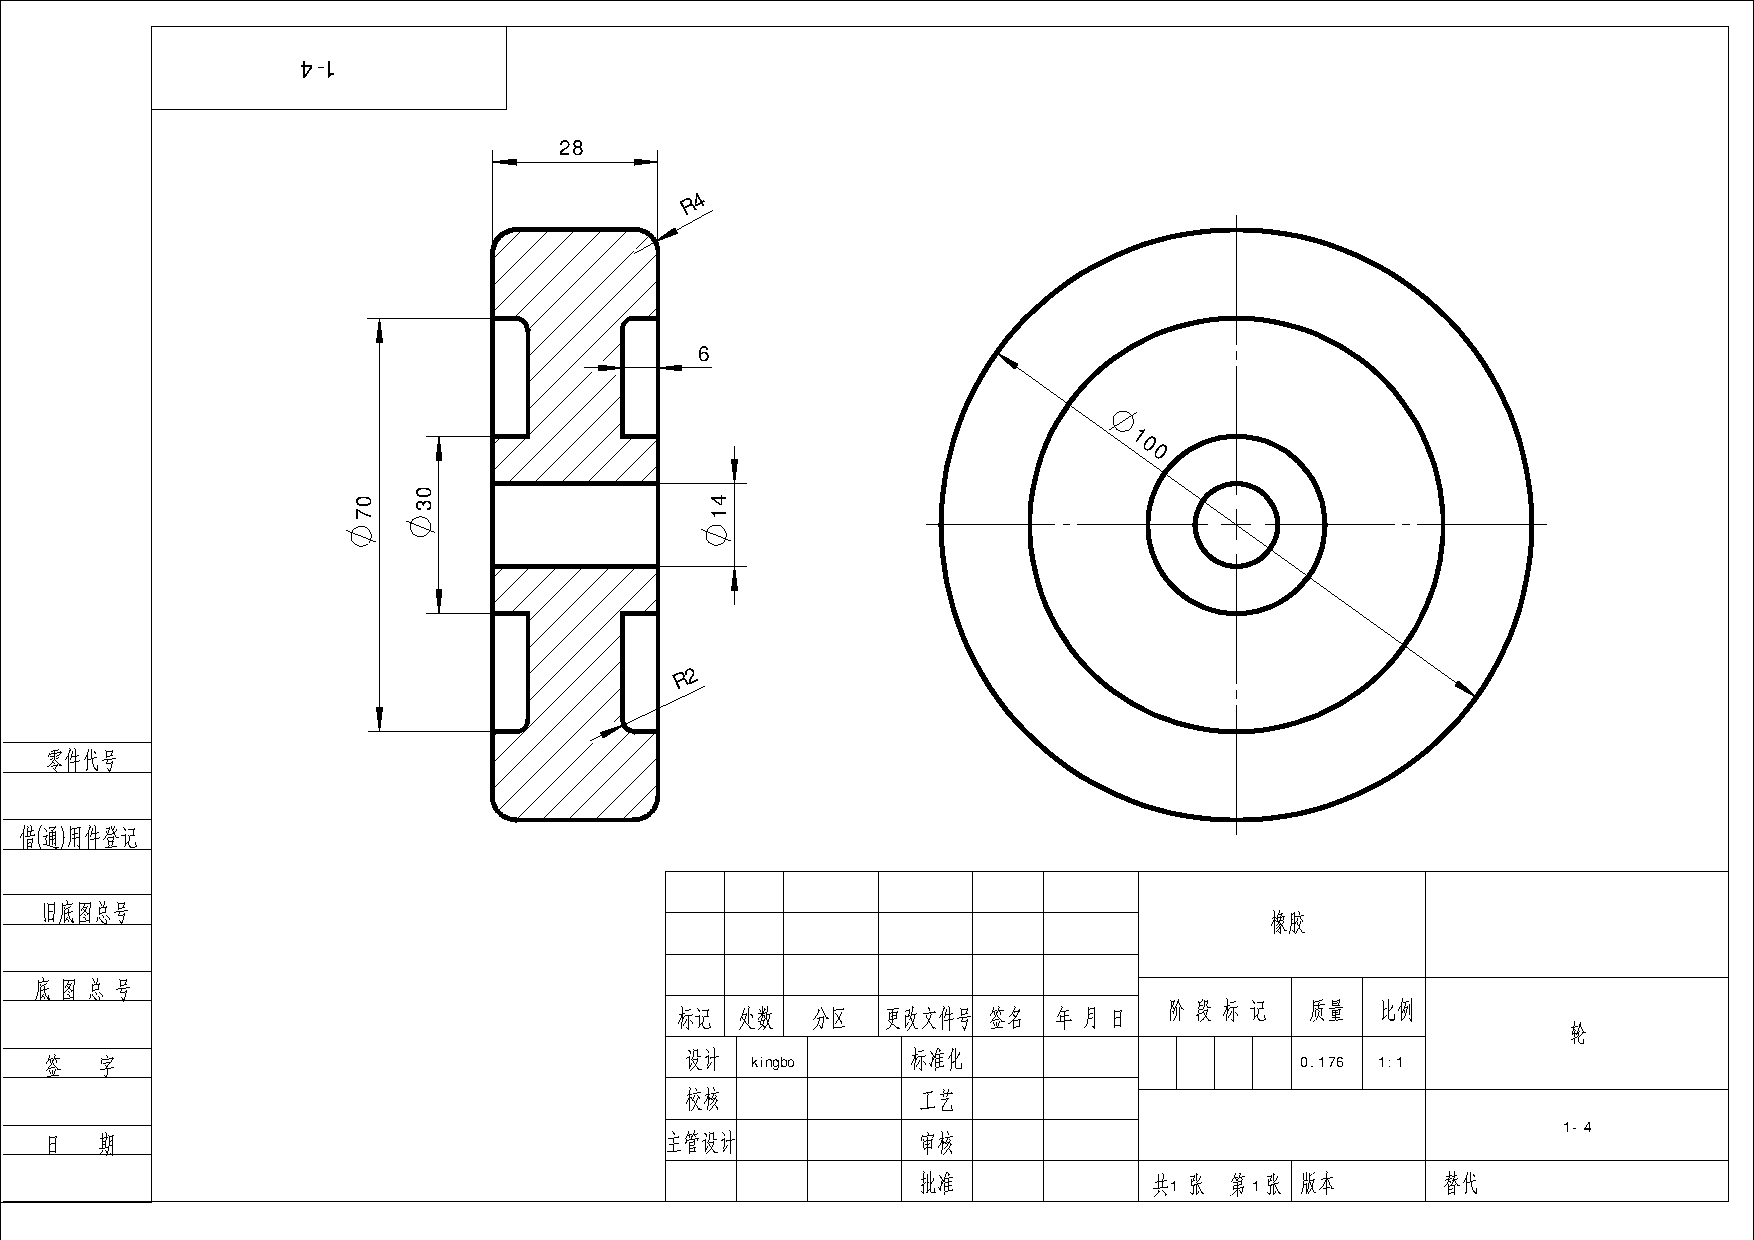
\includegraphics[scale=0.45]{xiaolunlun.pdf}
\caption{轮零件图}\label{fig:xiaolunlun.pdf}
\end{figure}

本章的目标是构建图\ref{fig:xiaolunlun.pdf}所示的小轮组轮零件的三维模型,并在此基础之上制作轮的零件图。因此本章重点讲解以下内容:
\begin{itemize}
\item 轮的三维模型构建
\item 剖视图的概念
\item 轮全剖视图的制作
\item 半径和直径尺寸的标注
\end{itemize}

\section{轮建模分析}
\subsection{实体建模方案}
\subsubsection{方案一}
根据制作图\ref{fig:xiaoluntaotong}所示套筒三维模型的经验,可以将图\ref{fig:xiaolunlun.pdf}所示的轮零件拆分为图\ref{fig:lunfenxi1.png}所示的套筒和\ref{fig:lunfenxi2.png}所示结构的组合。\ref{fig:lunfenxi2.png}所示结构又可以以此方式进一步简单为两个套筒的组合。这种简化方案的三维建模过程简单,难点主要在于各个组成部分的定位,需要利用套筒模型的轴心线的中点进行定位,才能够获得准确的模型。故需要绘制轴心辅助线,以利于组合定位。
\begin{figure}[htbp]
\centering
\subfloat[]{\label{fig:lunfenxi1.png}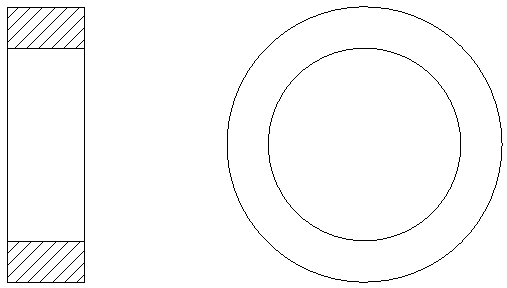
\includegraphics[scale=0.4]{lunfenxi1.png}}\hspace{20pt}
\subfloat[]{\label{fig:lunfenxi2.png}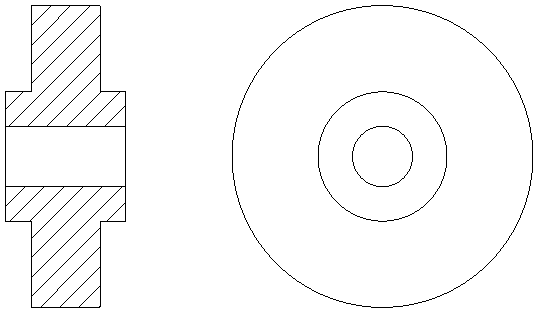
\includegraphics[scale=0.25]{lunfenxi2.png}}
\caption{轮实体建模方案一}
\end{figure}
\subsubsection{方案二}

注意到图\ref{fig:xiaolunlun.pdf}中的主视图不仅具有上下对称的特点,同时还具备上下对称的特性。故可以先构一半的模型,然后利用镜像来快速构建另一半模型。因此,图\ref{fig:xiaolunlun.pdf}所示的轮零件可以图\ref{fig:lunfenxi3.png}所示$\frac{1}{2}$长的套筒,然后减去图\ref{fig:lunfenxi4.png}所示的套筒,来获得图\ref{fig:lunfenxi5.png}所示模型,最后,利用镜像构建另一半模型。这种建模方案定位比较方便,不需要绘制用于定位的辅助线,构建方式也简单直接。为便于叙述,\ref{sec:lunjianmo}节 将图\ref{fig:lunfenxi3.png}所示的套筒称为被减套筒,图\ref{fig:lunfenxi4.png}所示的套筒称为减去套筒。
\begin{figure}[htbp]
\centering
\subfloat[]{\label{fig:lunfenxi3.png}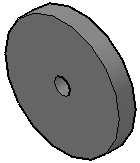
\includegraphics[scale=0.6]{lunfenxi3.png}}\hspace{20pt}
\subfloat[]{\label{fig:lunfenxi4.png}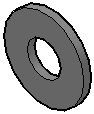
\includegraphics[scale=0.6]{lunfenxi4.png}}\hspace{20pt}
\subfloat[]{\label{fig:lunfenxi5.png}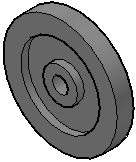
\includegraphics[scale=0.6]{lunfenxi5.png}}
\caption{轮实体建模方案二}
\end{figure}

当然,还存在其它的实体建模方案,这里就不一一赘述。读者有兴趣,可以逐尝用多种不同的构建方案进行三维模型构建,仔细体会每种组合方式的特点。
\subsection{旋转建模方案}

\begin{figure}[htbp]
\centering
\subfloat[]{\label{fig:lunfenxi6.png}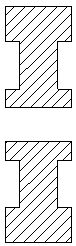
\includegraphics[scale=0.7]{lunfenxi6.png}}\hspace{40pt}
\subfloat[]{\label{fig:lunfenxi7.png}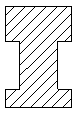
\includegraphics[scale=1]{lunfenxi7.png}}
\caption{轴旋转建模方案}
\end{figure}

基于图\ref{fig:xiaolunlianjiegan}所示连接杆的三维建模经验,图\ref{fig:xiaolunlun.pdf}所示的轮零件忽略圆角后具有图\ref{fig:lunfenxi6.png}所示的截面,因此可绘制图\ref{fig:lunfenxi7.png}所示的轮廓线来构成旋转特征面,并通过旋转的方式来完成模型的构建。这种建模方式也比较简单快捷。

\yaodian{尝用不同的方式构建模型,能有效提升灵活解决问题的能力。}
\endinput
\section{轮三维建模}\label{sec:lunjianmo}
在上节的分析中,轮的三维建模存在多种方式,本节将采用第二种实体建模方案,至于其它的建模方案读者可自行尝试。

\begin{procedure}
\item 切换视图方向为西南等轴测

为了方便观察三维建模结果,首先将AutoCAD的视图方向切换成西南等轴测。此时AutoCAD三维坐标系中的$x$和$y$坐标是位于水平面之中的。
\begin{lstlisting}
命令: -VIEW
输入选项 [?/删除(D)/正交(O)/恢复(R)/保存(S)/设置(E)/窗口(W)]: swiso
\end{lstlisting}

\item 切换坐标系为左视图方向

由于表征轮零件回转体特征的视图位于左视图之中,因此需要将将AutoCAD三维坐标系中$x$和$y$的位置切换至$W$面中,实现在不切换视图的方式下切换坐标系,需要用到用户坐标系命令。所谓用户坐标系(UCS)是指可以移动的坐标系,它是一种用于二维图形和三维建模的基本工具。它是相对于世界坐标系而言的。所谓世界坐标系(WCS)是用于定义图形中所有对象的位置和其他坐标系的固定坐标系。在AutoCAD中调用设置用户坐标系命令的方法有:

\begin{itemize}
\item 键盘输入UCS\index{ucs,用户坐标}
\item 【工具】
\includegraphics[scale=0.45]{ucstools.png}栏中的【UCS】
\includegraphics[scale=0.45]{ucs.png}
\end{itemize}

用户坐标系命令调用后,会提示当前的UCS坐标系名称,并要求指定新原点或选项。由于还没有构建好的模型,所以选择【Z轴(ZA)】选项。
\begin{lstlisting}
命令: UCS
当前 UCS 名称: *世界*
指定 UCS 的原点或 [面(F)/命名(NA)/对象(OB)/上一个(P)/视图(V)/世界(W)/X/Y/Z/Z 轴(ZA)] <世界>: za
\end{lstlisting}
选择ZA选项后,会提示指定新点,当前默认是(0,0,0),因此直接接受即可。
\begin{lstlisting}
指定新原点或 [对象(O)] <0,0,0>:
\end{lstlisting}
接下来,要求输入在正Z轴范围上指定点,此时需要将$z$轴置于水平面内因此,将$x$轴上的值设置为1,即输入(-1,0,0)。完成后系统的三维坐标系会由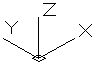
\includegraphics[scale=0.15]{hthreeaxis.png}状态改变为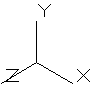
\includegraphics[scale=0.15]{wthreeaxis.png}状态。可以看出此时的$x$轴和$y$轴位于三维坐标平面中的$W$平面之中。
\begin{lstlisting}
在正 Z 轴范围上指定点 <0.0000,0.0000,1.0000>: -1,0,0
\end{lstlisting}

\item 构建被减套筒

由于需要采用镜像的方式构建轮零件的一半模型,因此只需要构建出一半的轮零件三维模型。首先构建的是$\phi 100$长14的圆柱体,结果如图\ref{fig:lunjianmo1.png} 所示。
\begin{lstlisting}
命令: CYLINDER
指定底面的中心点或 [三点(3P)/两点(2P)/切点、切点、半径(T)/椭圆(E)]:
指定底面半径或 [直径(D)]: 50
指定高度或 [两点(2P)/轴端点(A)]: 14
\end{lstlisting}
\begin{figure}[htbp]
\centering
\subfloat[]{\label{fig:lunjianmo1.png}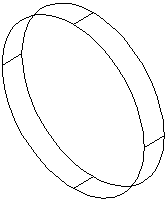
\includegraphics[scale=0.4]{lunjianmo1.png}}\hspace{20pt}
\subfloat[]{\label{fig:lunjianmo2.png}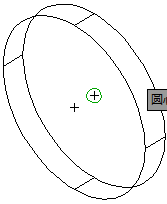
\includegraphics[scale=0.4]{lunjianmo2.png}}\hspace{20pt}
\subfloat[]{\label{fig:lunjianmo3.png}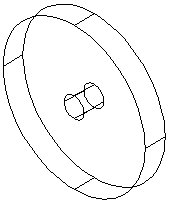
\includegraphics[scale=0.4]{lunjianmo3.png}}
\caption{被减套筒构建}
\end{figure}

构建$\phi 14$长14圆柱体时以图\ref{fig:lunjianmo2.png}所示的圆心作为圆柱体的底圆圆心。
\begin{lstlisting}
命令: CYLINDER
指定底面的中心点或 [三点(3P)/两点(2P)/切点、切点、半径(T)/椭圆(E)]:
指定底面半径或 [直径(D)] <50.0000>: 7
指定高度或 [两点(2P)/轴端点(A)] <14.0000>:
\end{lstlisting}

接下来,将$\phi 14$圆柱体从$\phi 100$圆体中减去,结果如图\ref{fig:lunjianmo3.png}所示。
\begin{lstlisting}
命令: SUBTRACT
选择要从中减去的实体、曲面和面域...
选择对象: 找到 1 个
选择对象:  选择要减去的实体、曲面和面域...
选择对象: 找到 1 个
选择对象:
\end{lstlisting}

\item 构建减去套筒

完成被减套筒的构建后,以图\ref{fig:lunjianmo4.png} 所示的圆为圆柱体底圆圆心构建$\phi 70$长6圆柱体。
\begin{lstlisting}
命令: CYLINDER
指定底面的中心点或 [三点(3P)/两点(2P)/切点、切点、半径(T)/椭圆(E)]:
指定底面半径或 [直径(D)] <7.0000>: 35
指定高度或 [两点(2P)/轴端点(A)] <14.0000>: -6
\end{lstlisting}

\begin{figure}[htbp]
\centering
\subfloat[]{\label{fig:lunjianmo4.png}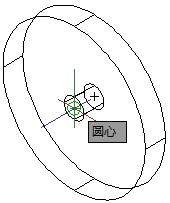
\includegraphics[scale=0.5]{lunjianmo4.png}}\hspace{40pt}
\subfloat[]{\label{fig:lunjianmo5.png}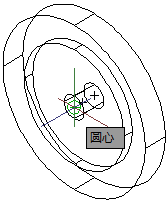
\includegraphics[scale=0.5]{lunjianmo5.png}}
\caption{减去套筒圆柱体构建}
\end{figure}

接下来,以图\ref{fig:lunjianmo5.png}所示圆心位置作为$\phi 30$长6圆柱体的底圆圆心。
\begin{lstlisting}
命令: CYLINDER
指定底面的中心点或 [三点(3P)/两点(2P)/切点、切点、半径(T)/椭圆(E)]:
指定底面半径或 [直径(D)] <35.0000>: 15
指定高度或 [两点(2P)/轴端点(A)] <-6.0000>:
\end{lstlisting}


\yaodian{使用负数高度值作为圆柱体的高度,将以$z$轴的反方向构建圆柱体。}

在构建减去套筒圆柱体时要选择图\ref{fig:lunjianmo6.png}所示圆柱作为要从中减去的实体,选择图\ref{fig:lunjianmo7.png}所示圆柱体作为要减去的实体。
\begin{lstlisting}
命令: SUBTRACT
选择要从中减去的实体、曲面和面域...
选择对象: 找到 1 个
选择对象:  选择要减去的实体、曲面和面域...
选择对象: 找到 1 个
选择对象:
\end{lstlisting}

\begin{figure}[htbp]
\centering
\subfloat[]{\label{fig:lunjianmo6.png}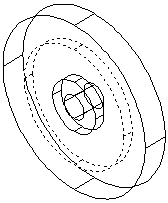
\includegraphics[scale=0.5]{lunjianmo6.png}}\hspace{40pt}
\subfloat[]{\label{fig:lunjianmo7.png}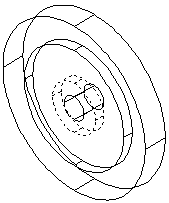
\includegraphics[scale=0.5]{lunjianmo7.png}}
\caption{减去套筒差集过程}
\end{figure}
\item 套筒组合

\begin{lstlisting}
命令: SUBTRACT
选择要从中减去的实体、曲面和面域...
选择对象: 找到 1 个
选择对象:  选择要减去的实体、曲面和面域...
选择对象: 找到 1 个
选择对象:
\end{lstlisting}

\begin{figure}[htbp]
\centering
\subfloat[]{\label{fig:lunjianmo8.png}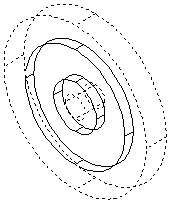
\includegraphics[scale=0.5]{lunjianmo8.png}}\hspace{40pt}
\subfloat[]{\label{fig:lunjianmo9.png}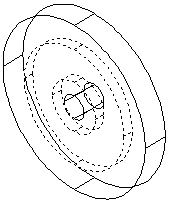
\includegraphics[scale=0.5]{lunjianmo9.png}}
\caption{半轮零件模型构建}
\end{figure}

要构建图\ref{fig:lunfenxi5.png}所示的半轮零件模型,需要被减套筒中去掉减去套筒部分,因此要选择图\ref{fig:lunjianmo8.png}所示的虚线实体作为要从中减去的实体,选择图\ref{fig:lunjianmo9.png}所示的虚线实体作为要减去的实体。

\item 倒圆角边

完成套筒的组合后,需要构建半轮零件的圆角边。以便于一起进行镜像操作。在AutoCAD完成圆角边构建的命令是圆角边,其调用方法有:
\begin{itemize}
\item 键盘输入filletedge\index{filletedge,圆角边}
\item 【修改】$\rightarrow $【实体编辑】$\rightarrow $【圆角边】
\item 【实体编辑】
\includegraphics[scale=0.45]{solidedittools}工具栏中的【圆角边】
\includegraphics[scale=0.45]{filletedge}图标
\end{itemize}

\begin{figure}[htbp]
\centering
\subfloat[]{\label{fig:lunjianmo10.png}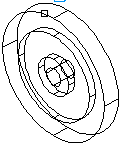
\includegraphics[scale=0.6]{lunjianmo10.png}}\hspace{20pt}
\subfloat[]{\label{fig:lunjianmo11}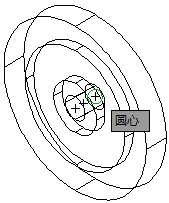
\includegraphics[scale=0.6]{lunjianmo11.png}}\hspace{20pt}
\subfloat[]{\label{fig:lunjianmo12}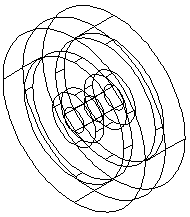
\includegraphics[scale=0.6]{lunjianmo12}}
\caption{圆角边操作过程}
\end{figure}

圆角边命令调用后,会提示当前的半径值。如果当前的半径值与实际需求值是一致的,则可以直接操作,不用设置圆角半径;若不一致则应当设置圆角半径。此例中,圆角半径与当前值不一致,因此需要进行设置。
\begin{lstlisting}
命令:  FILLETEDGE
半径 = 1.0000
\end{lstlisting}

要设置圆角边的半径值,需要使用【半径(R)】选项,输入半径选项后会提示输入圆角半径值。
\begin{lstlisting}
选择边或 [链(C)/环(L)/半径(R)]: r
输入圆角半径或 [表达式(E)] <1.0000>: 4
\end{lstlisting}
完成圆角半径设置后,按图\ref{fig:lunjianmo10.png}所示选择要倒角的边,选择完成后会生成\ref{fig:lunjianmo11}所示的圆角边预览结果。
\begin{lstlisting}
选择边或 [链(C)/环(L)/半径(R)]:
\end{lstlisting}

由于只一条$R4$的圆角边,所以直接结束选择并接受圆角结果,最终效果如图\ref{fig:lunjianmo12}所示。
\begin{lstlisting}
选择边或 [链(C)/环(L)/半径(R)]:
已选定 1 个边用于圆角。
按 Enter 键接受圆角或 [半径(R)]:
\end{lstlisting}

接下来按图\ref{fig:lunjianmo13}所示选择边来完成$R2$圆角边的构建,结果如图\ref{fig:lunjianmo14}所示。
\begin{lstlisting}
命令:  FILLETEDGE
半径 = 4.0000
选择边或 [链(C)/环(L)/半径(R)]: r
输入圆角半径或 [表达式(E)] <4.0000>: 2
选择边或 [链(C)/环(L)/半径(R)]:
选择边或 [链(C)/环(L)/半径(R)]:
已选定 1 个边用于圆角。
按 Enter 键接受圆角或 [半径(R)]:
\end{lstlisting}

\begin{figure}[htbp]
\centering
\subfloat[]{\label{fig:lunjianmo13}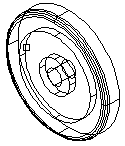
\includegraphics[scale=0.6]{lunjianmo13}}\hspace{40pt}
\subfloat[]{\label{fig:lunjianmo14}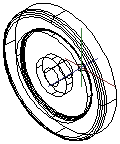
\includegraphics[scale=0.6]{lunjianmo14}}
\caption{$R2$圆角边操作}
\end{figure}
\item 镜像

至此已经完成一半的轮零件三维模型的制作,另一半也可以用上面的步骤来完成,但这样效率过低,也违背了初忠。最快的方法是使用三维镜像来完成。在AutoCAD中调用三维镜像的的方法有:
\begin{itemize}
\item 键盘输入mirror3d\index{mirror3d,三维镜像}
\item 【修改】$\rightarrow $【三维操作】$\rightarrow $【三维镜像】
\end{itemize}

三维镜像命令调用后,会提示选择对象,此时模型空间中仅有一个对象,因此用鼠标直接选取该对象,选择后如图\ref{fig:lunjianmo15}所示。
\begin{lstlisting}
命令: mirror3d
选择对象: 找到 1 个
选择对象:
\end{lstlisting}

\begin{figure}[htbp]
\centering
\subfloat[]{\label{fig:lunjianmo15}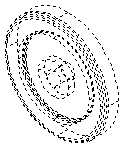
\includegraphics[scale=0.6]{lunjianmo15}}\hspace{20pt}
\subfloat[]{\label{fig:lunjianmo16}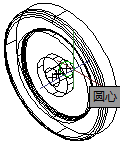
\includegraphics[scale=0.6]{lunjianmo16}}\hspace{20pt}
\subfloat[]{\label{fig:lunjianmo17}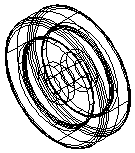
\includegraphics[scale=0.6]{lunjianmo17}}
\caption{三维镜像过程}
\end{figure}
接下来,命令要求以三点方式指定镜像平面,经过观察可知图\ref{fig:lunjianmo15}所示模型的镜像平面位于右端面,并助该镜像平面与$xy$平面平行,因此应该选择【XY平面(XY)】选项。
\begin{lstlisting}
指定镜像平面 (三点) 的第一个点或
  [对象(O)/最近的(L)/Z 轴(Z)/视图(V)/XY 平面(XY)/YZ 平面(YZ)/ZX 平面(ZX)/三点(3)] <三点>: xy
\end{lstlisting}

然后,命令提示指定XY平面上的点,此时选择图\ref{fig:lunjianmo16}所示的选定的圆心作为XY平面上的点。
\begin{lstlisting}
指定 XY 平面上的点 <0,0,0>:
\end{lstlisting}
最后命令示确认是否删除源对象,默认是否,故直接确认。完成后结果如图\ref{fig:lunjianmo17}所示。
\begin{lstlisting}
是否删除源对象?[是(Y)/否(N)] <否>:
\end{lstlisting}

\item 合成轮零件三维模型

镜像完成后,轮零件三维模型还不是一个整体,因此需要运用并集命令将两个实例合并为一个实体。
\begin{lstlisting}
命令: UNION
选择对象: 指定对角点: 找到 2 个
选择对象:
\end{lstlisting}

\item 切换视觉样式为灰度

合并完成后,将视觉样式切换为灰度,即可看来图\ref{fig:lunjianmo18} 所示的轮零件三维模型结果。
\begin{lstlisting}
命令: VSCURRENT
输入选项 [二维线框(2)/线框(W)/隐藏(H)/真实(R)/概念(C)/着色(S)/带边缘着色(E)/灰度(G)/勾画(SK)/X 射线(X)/其他(O)] <二维线框>: g
\end{lstlisting}

\begin{figure}[htbp]
\centering
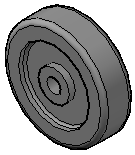
\includegraphics[scale=0.9]{lunjianmo18}
\caption{轮零件三维模型}\label{fig:lunjianmo18}
\end{figure}
\item 保存轮零件三维模型

最后,将完成的轮零件三维模型以“轮.dwg"的文件名予以保存。
\end{procedure}
\endinput
\section{轮零件图制作}

\endinput
%\section{标题栏、尺寸、文字}

\endinput
\endinput